\section{Approach}

This project consists of three key stages, each with specific goals that contribute to the overall aim of developing a robust and adaptable Multi-Agent System (MAS) for managing autonomous vehicles at road intersections. 
The stages are as follows:

\begin{figure}[H]
    \centering
    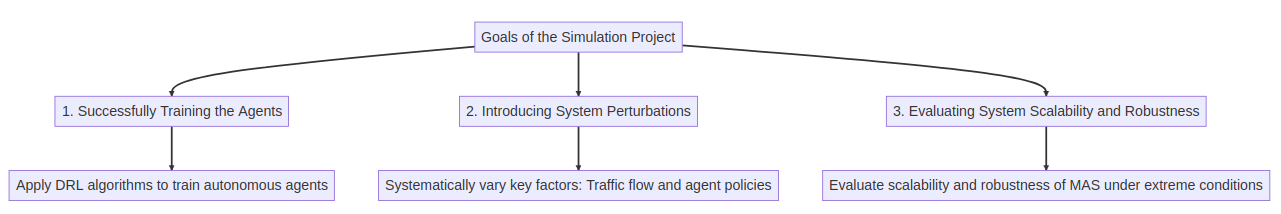
\includegraphics[height=0.12\textheight]{images/goals.png} 
    \caption{Project Methodology}
\end{figure}

\begin{enumerate}
    \item \textbf{Successfully train the agents}

       In this phase, we will apply selected Deep Reinforcement Learning (DRL) algorithms to train autonomous agents in navigating a road intersection.
       
       The agents will learn to make decisions related to intersection crossing order and speed control, with the goal of optimizing traffic flow and avoiding collisions.
           
    \item \textbf{Introducing System Perturbations}
    
   At this stage, the goal is to understand how our different agent policies (policy refers to the strategy/mapping in each agent from state to action) perform when presented with different environment configurations. When it comes to the environment, we tested with two different traffic flow configurations, 
   which we defined as \textbf{sparse} (4 ego vehicles, few other vehicles) or \textbf{dense} (4 ego vehicles, many other vehicles). 
   The goal is to understand if the difference in configuration will alter the algorithm's performance and/or if any of the algorithms are more robust to the changes than others.
       

       
    \item \textbf{Evaluate system scalability and robustness}

    Having trained our learning models, we can load them into the environment and use the approximated policy to make decisions. 
    We run a select number of simulations use this policy and gather metrics from the environment, 
    which are used to compare and evaluate each of the learning algorithms.
\end{enumerate}


\section{Successfully train the agents}


\subsection{Reinforcement Learning Training Process}

\begin{figure}[H]
    \centering
    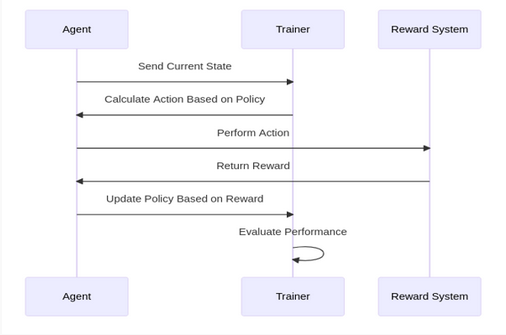
\includegraphics[height=0.25\textheight]{images/train.png} 
    \caption{RL Training Process Sequence}
\end{figure}

The Training Process Sequence can be described as follows:

\subsubsection{1.Initialization}
\begin{itemize}
    \item \textbf{Environment Setup}: An environment is defined (e.g., a traffic intersection using Highway-Env), which provides the observation and action spaces. The environment simulates the interactions of agents and their surroundings.
    \item \textbf{Observation Space}: This defines what the agent perceives at each timestep. For example:
    \begin{itemize}
        \item In the traffic environment, the observation may include a grayscale image of the environment (shape: \((128, 64)\)), stacked over 4 frames to provide temporal context.
        \item The observations are preprocessed to include essential information, such as vehicle positions, velocities, and surrounding traffic.
    \end{itemize}
    \item \textbf{Action Space}: The possible actions an agent can take at each timestep, such as accelerating, braking, or changing lanes in the traffic context.
    \item \textbf{Reward Function}: Rewards guide the agent's learning by providing feedback. The reward is carefully designed to encourage desired behaviors, such as:
    \begin{itemize}
        \item Minimizing travel time.
        \item Avoiding collisions.
        \item Yielding or cooperating with other agents.
    \end{itemize}
\end{itemize}

\subsubsection{2.Agent Initialization}
\begin{itemize}
    \item An RL agent, such as one trained using the Deep Q-Network (DQN) or Proximal Policy Optimization (PPO) algorithm, is instantiated.
    \item The agent interacts with the environment through a defined policy. For example:
    \begin{itemize}
        \item \textbf{DQN}: Uses a neural network to approximate the Q-function, mapping states and actions to expected future rewards.
        \item \textbf{PPO}: Optimizes the policy directly, ensuring stable updates with a clipped objective function.
    \end{itemize}
\end{itemize}

\subsubsection{3.Interaction with the Environment}
At each timestep:
\begin{itemize}
    \item \textbf{Observation}: The agent observes the current state of the environment.
    \item \textbf{Action Selection}: Based on the observation, the agent selects an action using its policy (e.g., an \(\epsilon\)-greedy policy in DQN).
    \item \textbf{Environment Response}: The environment executes the action and provides:
    \begin{itemize}
        \item The next state.
        \item A reward signal.
        \item A flag indicating whether the episode has ended.
    \end{itemize}
\end{itemize}

\subsubsection{4.Experience Storage}
\begin{itemize}
    \item The agent stores experiences as tuples \((s, a, r, s')\) in a replay buffer (for DQN) or uses the trajectory for on-policy updates (PPO).
\end{itemize}

\subsubsection{5.Policy Optimization}
\begin{itemize}
    \item \textbf{DQN}:
    \begin{itemize}
        \item A mini-batch of experiences is sampled from the replay buffer.
        \item The Q-function is updated using the Bellman equation:
        \begin{equation}
        Q(s, a) \leftarrow r + \gamma \max_{a'} Q(s', a')
        \end{equation}
        \item The agent minimizes the temporal difference error between predicted and target Q-values.
    \end{itemize}
    \item \textbf{PPO}:
    \begin{itemize}
        \item The agent computes the advantage function to estimate the relative value of actions.
        \item Policy and value networks are optimized using the PPO loss:
        \begin{equation}
        L(\theta) = \mathbb{E}_t\left[ \min \left( r_t(\theta) A_t, \text{clip}(r_t(\theta), 1-\epsilon, 1+\epsilon) A_t \right) \right]
        \end{equation}
        \item The clipping ensures stable updates.
    \end{itemize}
\end{itemize}

\subsubsection{6.Evaluation and Improvement}
\begin{itemize}
    \item At regular intervals, the agent's policy is evaluated in the environment to assess its performance.
    \item Metrics such as mean reward and train loss are used to gauge improvement.
    \item The best-performing model is saved during training for deployment.
\end{itemize}

\subsubsection{7.End of Training}
\begin{itemize}
    \item After reaching the desired number of training timesteps, the final policy is saved.
    \item Post-training evaluations are conducted to ensure the agent generalizes well to unseen scenarios.
\end{itemize}


\newpage

\subsection{Practical Training Implementation - Configuration}

The training of each agent using the "standard" DQN and PPO algorithms was conducted with \textbf{Stable-Baselines3}\cite{stable-baselines3} within 
a custom multi-agent environment created using the \textbf{Highway-Env} library.

\subsubsection{DQN and PPO with CnnPolicy }

\subsubsection{1.Initialization}

Environment Setup, Observation Space (Python coded): 

\begin{lstlisting}[style=python]
    env = make_vec_env(
        "intersection-v0", 
        n_envs=n_cpu, 
        vec_env_cls=SubprocVecEnv, 
        env_kwargs={
            'config':{
                'initial_vehicle_count': 10,
                'controlled_vehicles': 4,
                'destination': 'o1',
                "observation": {
                    "type": "GrayscaleObservation",
                    "observation_shape": (128, 64),
                    "stack_size": 4,
                    "weights": [0.2989, 0.5870, 0.1140],  # weights for RGB conversion
                    "scaling": 1.75,
                },
            },
        }
    )
\end{lstlisting}

Each environment comes with a default observation, which can be changed or customised using environment configurations. 
In the intersection environment, in order to use the images needed for CNN, the observation type must be defined as \textit{GrayscaleObservation}.

The \textit{GrayscaleObservation} is a \( W \times H \) grayscale image of the scene, where \( W \) and \( H \) are set with the \textit{observation\_shape} parameter. 
The RGB to grayscale conversion is a weighted sum configured by the \textit{weights} parameter. 
Several images can be stacked with the \textit{stack\_size} parameter.



The \textbf{Action Space} is configured as:

\begin{lstlisting}[style=python]
'action': {'lateral': False,
            'longitudinal': True,
            'target_speeds': [0, 4.5, 9],
            'type': 'DiscreteMetaAction'},
\end{lstlisting}

In the default configuration of the intersection environment, only the speed is controlled by the agent, 
while the lateral control of the vehicle is automatically performed by a steering controller to track a desired lane.

So, in this environment the Action Space is defined as:

\begin{lstlisting}[style=python]
ACTIONS= {
        0: 'IDLE',
        1: 'SLOWER',
        2: 'FASTER'
    }
\end{lstlisting}

The \textbf{Reward Function} is focused focus on two features: a vehicle should:

    progress quickly on the road;

    avoid collisions.

Thus, the reward function is composed of a velocity term and a collision term:
\[
R(s,a) = a \left( \frac{v - v_{\min}}{v_{\max} - v_{\min}} \right) - b \text{ collision}
\]

where \( v \), \( v_{\min} \), and \( v_{\max} \) are the current, minimum, and maximum speed of the ego-vehicle respectively, and \( a \), \( b \) are two coefficients.

In practical terms the following rewards are used in this environment:
\begin{lstlisting}[style=python]
    'arrived_reward': 1,
    'collision_reward': -5,
    'high_speed_reward': 1
\end{lstlisting}

Being the final episode reward calculated as an average of the reward of all controlled agents.

\subsubsection{2.1 - Agent Initialization for DQN algorithm using CnnPolicy}

The following parameters have been used in the training processes with CnnPolicy :

\begin{lstlisting}[style=python]
    model = DQN(
        "CnnPolicy",
        env,
        learning_rate=5e-4,
        buffer_size=15000,
        learning_starts=200,
        batch_size=32,
        gamma=0.8,
        train_freq=1,
        gradient_steps=1,
        target_update_interval=50,
        exploration_fraction=0.7,
        verbose=2,
        tensorboard_log=model_dir,
    )
\end{lstlisting}

\subsubsection{2.2 - Agent Initialization for PPO algorithm using CnnPolicy}

\begin{lstlisting}[style=python]
    batch_size = 64
    model = PPO(
        "CnnPolicy",
        env,
        n_steps=batch_size * 12 // n_cpu,
        batch_size=batch_size,
        n_epochs=10,
        learning_rate=3e-4,
        gamma=0.9,
        verbose=2,
        tensorboard_log=model_dir,
    )
\end{lstlisting}

\subsubsection{DQN and PPO with MlpPolicy }

\subsubsection{1.Initialization}

Environment Setup, Observation Space (Python coded): 

\begin{lstlisting}[style=python]
    env = make_vec_env(
        "intersection-v0", 
        n_envs=n_cpu, 
        vec_env_cls=SubprocVecEnv, 
        env_kwargs={
            'config':{
                'vehicles_count': 10,
                'controlled_vehicles': 4,
                'destination': 'o1',
            },
        }
    )

\end{lstlisting}

The MlpPolicy needs a different type of observations: \textit{Kinematics}.

The \textit{KinematicObservation} is a  a \( V \times F \) array  and that describes a list of \( V \) nearby vehicles by a set of features of size  \( F \)
listed in the "features" configuration field. In this particular case we are using:

\begin{lstlisting}[style=python]
'observation': {'absolute': True,
'features': ['presence',
             'x',
             'y',
             'vx',
             'vy',
             'cos_h',
             'sin_h'],
'features_range': {'vx': [-20, 20],
                   'vy': [-20, 20],
                   'x': [-100, 100],
                   'y': [-100, 100]},
'type': 'Kinematics',
}
\end{lstlisting}

where: 

\textit{presence}:Disambiguate agents at 0 offset from non-existent agents.

\textit{x} and \textit{y}: World offset of ego vehicle or offset to ego vehicle on the x and y axis.

\textit{vx} and \textit{vy}: Velocity on the x and y axis of vehicle.

\textit{cos\_h} and \textit{sin\_h}: Trigonometric heading of vehicle.


Which produces an observation array similar to the one represented in the table bellow:

\begin{table}[h!]
    \centering
    \begin{tabular}{|c|c|c|c|c|c|c|c|}
    \hline
    \textbf{Vehicle} & \textbf{presence} & \textbf{x} & \textbf{y} & \textbf{vx} & \textbf{vy} & \textbf{cos\_h} & \textbf{sin\_h} \\ \hline
    ego-vehicle & 1 & 5.0  & 4.0  & 15.0  & 0   & 1  & 0 \\ \hline
    vehicle 1  & 1 & -10.0 & 4.0  & 12.0  & 0   & 1  & 0 \\ \hline
    vehicle 2  & 1 & 13.0  & 8.0  & 13.5  & 0   & 1  & 0 \\ \hline
    ...         & ...   & ...  & ...   & ... & ... & ...& ... \\ \hline
    vehicle V  & 1 & 22.2  & 10.5 & 18.0  & 0.5 & 1  & 0 \\ \hline
    \end{tabular}
    \caption{Example of \textit{Kinematic} observation }
    \label{tab:vehicles}
\end{table}

 The Action Space and Reward Function are similar to those used in the \textit{CnnPolicy} 
    

 \subsubsection{2.1 - Agent Initialization for DQN algorithm using MlpPolicy}

 \begin{lstlisting}[style=python]
    model = DQN(
        "MlpPolicy",
        env,
        learning_rate=3e-4,
        buffer_size=15000,
        learning_starts=200,
        batch_size=32,
        gamma=0.8,
        train_freq=1,
        gradient_steps=1,
        target_update_interval=50,
        exploration_fraction=0.5,
        verbose=2,
        tensorboard_log=model_dir
    )
\end{lstlisting}

\subsubsection{2.2 - Agent Initialization for PPO algorithm using MlpPolicy}

\begin{lstlisting}[style=python]
    batch_size = 64
    model = PPO(
        "MlpPolicy",
        env,
        n_steps=batch_size * 12 // n_cpu,
        batch_size=batch_size,
        n_epochs=10,
        learning_rate=3e-4,
        gamma=0.9,
        verbose=2,
        tensorboard_log=model_dir,
    )
\end{lstlisting}

\subsubsection{DQN with Social Attention}

Configuration/Implementation based off \textit{rl-agents} GitHub Repository\cite{rl-agents}.
\subsubsection{1.Initialization}

Environment Setup, Observation Space (JSON encoded): 

\begin{lstlisting}[style=json]
{
    "id": "intersection-v0",
    "import_module": "highway_env",
    "observation": {
        "type": "Kinematics",
        "vehicles_count": 15,
        "features": ["presence", "x", "y", "vx", "vy", "cos_h", "sin_h"],
        "features_range": {
            "x": [-100, 100],
            "y": [-100, 100],
            "vx": [-10, 10],
            "vy": [-10, 10]
        },
        "absolute": true,
        "order": "shuffled"
    },
    "initial_vehicle_count": 0,
    "vehicles_count": 0,
    "controlled_vehicles": 4,
    "destination": "o1"
}

\end{lstlisting}

The Social Attention also uses \textit{Kinematics} observations.

The Action Space and Reward Function are similar to the other approaches. 
    

\subsubsection{2. Agent Initialization}

The agent used was the \textit{ego\_attention} with 2 heads:

 \begin{lstlisting}[style=json]
{
    ...
    
    "model": {
        "type": "EgoAttentionNetwork",
        "embedding_layer": {
            "type": "MultiLayerPerceptron",
            "layers": [64, 64],
            "reshape": false,
            "in": 7
        },
        "others_embedding_layer": {
            "type": "MultiLayerPerceptron",
            "layers": [64, 64],
            "reshape": false,
            "in": 7
        },
        "self_attention_layer": null,
        "attention_layer": {
            "type": "EgoAttention",
            "feature_size": 64,
            "heads": 2
        },
        "output_layer": {
            "type": "MultiLayerPerceptron",
            "layers": [64, 64],
            "reshape": false
        }
    }
}
\end{lstlisting}

The embedding layers are two parallel MLPs with identical structures that each take 7-dimensional inputs representing vehicle states. These layers encode the features of both the ego vehicle and surrounding vehicles separately, though they share weights.
At the core is an attention layer implemented as an \textit{EgoAttention} mechanism with 2 attention heads.
The final output layer uses an MLP to decode the attention-processed features and produce Q-values for the available actions.

\subsubsection{Decentralized Social Influence DQN}

As for decentralized training, each agent is represented by its own network (and therefore optimizer, during training). This means that each agent's network is being fitted only to its own actions, rewards and observations, rather than their collective counterparts. This approach can benefit training because when using the collective reward and observation, centralized networks might not be able to capture small changes in actions for each agent. Furthermore, this in turn allows us to use Social Influence, a concept in which each agent's behavior is influenced by others, which we will further explain. 

The key concept is that we are using this neural network as a universal function approximator in order to approximate our theoretical $Q$ function, which we could use to pick the maximum value action for each state. We assume the fact that every $Q$ function obeys the \textit{Bellman Equation}:
\[
Q^\pi(s, a) = r + \gamma Q^\pi(s', \pi(s'))
\]
From this, we get the temporal difference error, $\delta$, which is what we attempt to minimize:
\[
\delta = Q(s, a) - \left(r + \gamma \max_{a'} Q(s', a')\right)
\]

The training pipeline for this approach follows closely \cite{pytorchrltutorial}. Each agent is represented by its own policy network and target network. We select actions according to an epsilon greedy policy, using Replay Memory to store transitions of the type \textit{(State, Action, Next State, Reward}. By obtaining a batch of these transitions for each autonomous agent, we optimize the network by minimizing the \textit{Huber Loss} calculated with respect to the previously mentioned $delta$:

\[
L = \frac{1}{|B|} \sum_{(s, a, s', r) \in B} L(\delta),
\]
where
\[
L(\delta) =
\begin{cases} 
\frac{1}{2}\delta^2 & \text{for } |\delta| \leq 1, \\
|\delta| - \frac{1}{2} & \text{otherwise}.
\end{cases}
\]

where $(s, a, s', r)$ is a single transition.

Having succesfully achieve decentralized training, the next step would be to implemented some kind of social mechanism, given that the agent's have to learn to respond to each other's behavior, in particular in an road intersection scenario. We chose to implement what is known as the \textit{Basic Social Influence} mechanism from \cite{jaques2019social}, that shifts agent's rewards using counterfactuals, so that it becomes $r^k_t = \alpha e^k_t + \beta c^k_t$ where $e^k_t$ is the extrinsic or environmental reward, and $c^k_t$ is the causal influence reward.  Essentially, agent \textit{k} asks the question: “How would \textit{j’s} action change if I had acted differently in this situation?”. This causal influence rewards is obtained by calculating the divergence between the marginal policy of j (if \textit{j} did not consider \textit{k}) and the conditional policy of \textit{j} (when \textit{j} does consider \textit{k}).

\begin{figure}[h]
    \centering
    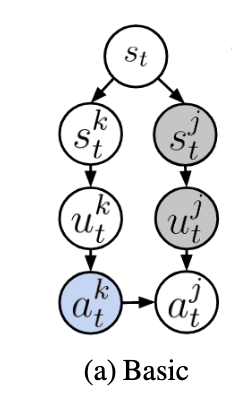
\includegraphics[scale=0.5]{images/social_influence.png}
    \caption{Chain of social influence}
    \label{fig:social influence}
\end{figure}



\subsection{Practical Training Implementation - Execution and Results}

The previously configured models were trained for a minimum of 1 million timesteps or until the average reward reached its maximum value. 
At regular intervals, the agent's policy was evaluated within the environment to assess its performance,
and the model was saved whenever the metrics improved. 
Metrics such as mean reward and training loss were used to measure progress.

The training process was monitored using TensorBoard. 
For each training session, the evolution of the average reward and the train loss were displayed. 
Below are the logs of these processes:


\subsubsection{DQN}

1. DQN with CnnPolicy

\begin{figure}[H]
    \centering
    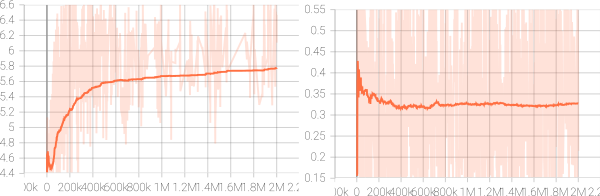
\includegraphics[height=0.20\textheight]{images/dqn_cnn.png} 
    \caption{DQN with CnnPolicy training Log - Average Reward and Train Loss Evolution}
\end{figure}


2. DQN with MlpPolicy

\begin{figure}[H]
    \centering
    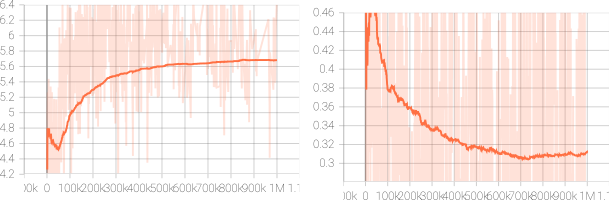
\includegraphics[height=0.20\textheight]{images/dqn_mlp.png} 
    \caption{DQN with MlpPolicy training Log - Average Reward and Train Loss Evolution}
\end{figure}

3. DQN with Social Attention

\begin{figure}[H]
    \centering
    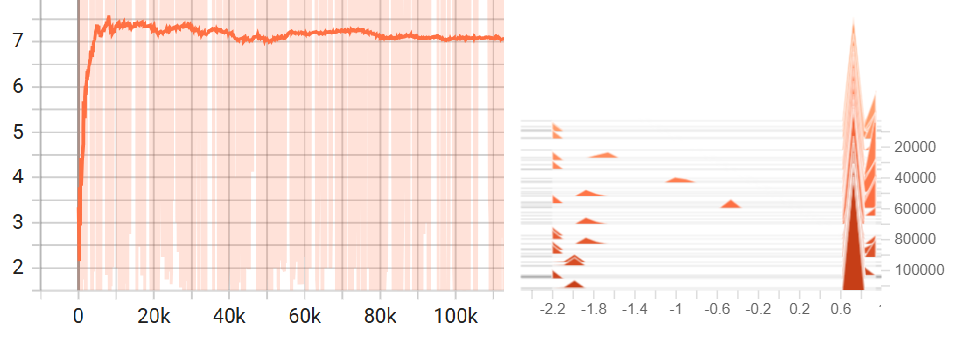
\includegraphics[height=0.20\textheight]{images/dqn_sa.png} 
    \caption{DQN with Social Attention training Log - Average Reward Evolution and its 3D View.}
\end{figure}

\subsubsection{PPO}

1. PPO with CnnPolicy

\begin{figure}[H]
    \centering
    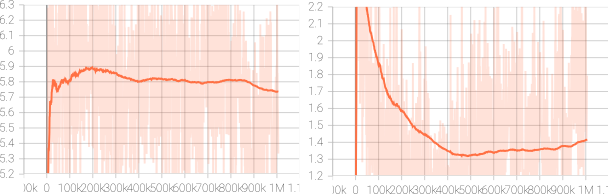
\includegraphics[height=0.20\textheight]{images/ppo_cnn.png} 
    \caption{PPO with CnnPolicy training Log - Average Reward and Train Loss Evolution}
\end{figure}



2. PPO with MlpPolicy

\begin{figure}[H]
    \centering
    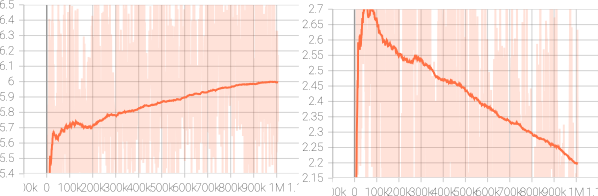
\includegraphics[height=0.20\textheight]{images/ppo_mlp.png} 
    \caption{PPO with MlpPolicy training Log - Average Reward and Train Loss Evolution}
\end{figure}


Decentralized Social Influence DQN


\begin{figure}[h]
    \centering
    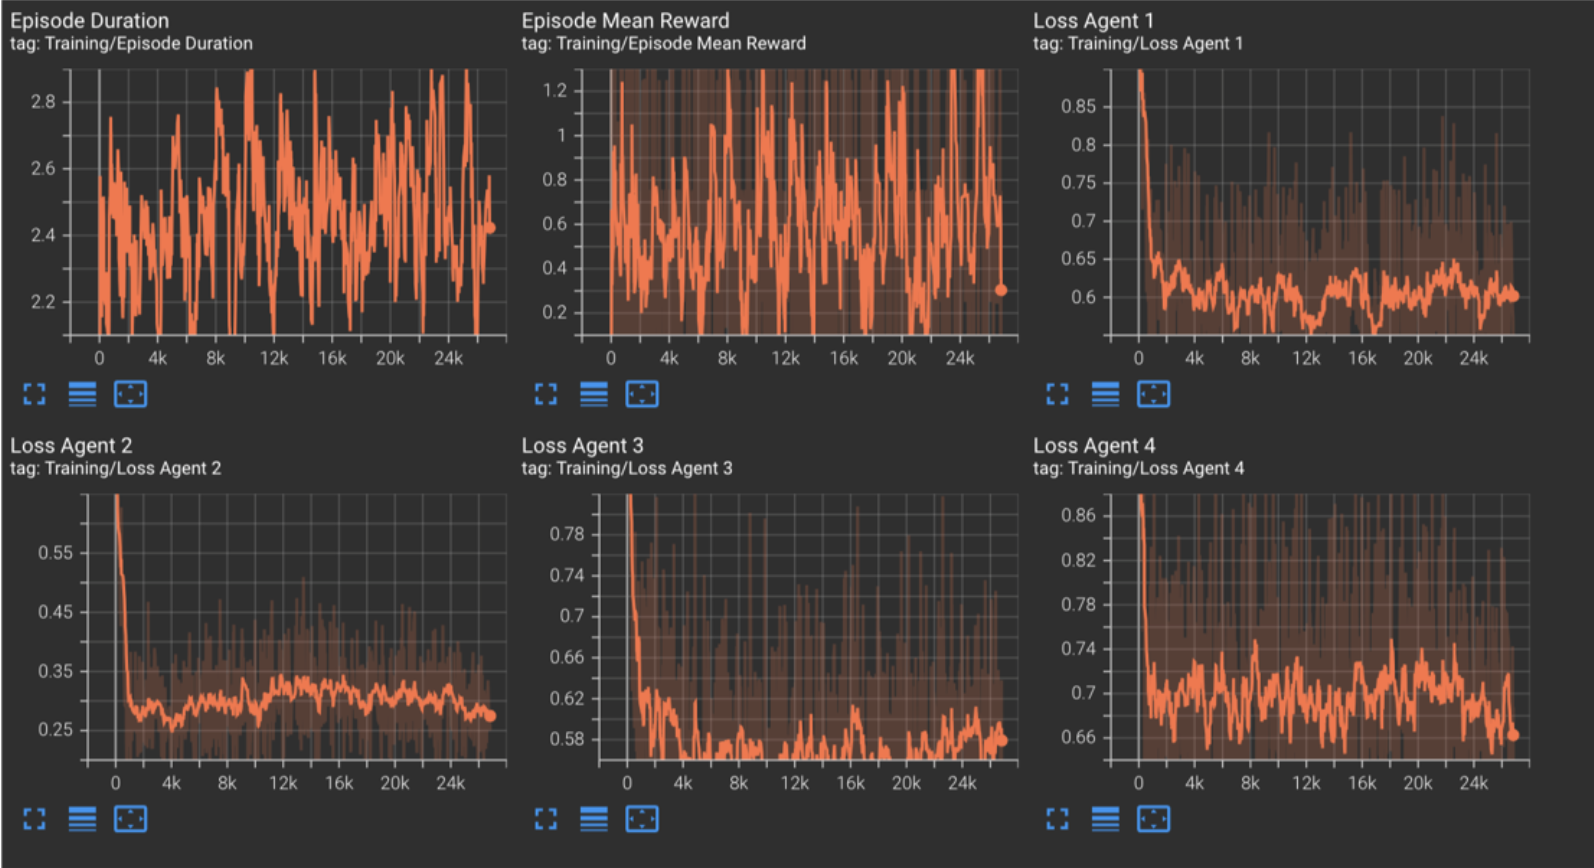
\includegraphics[scale=0.5]{images/dqn_SI_metrics.png}
    \caption{Social Influence Train Logs}
    \label{fig:social influence}
\end{figure}


\section{Introducing System Perturbations}

\subsection{Pipeline for Agent Policy Evaluation}

The primary goal of this study is to understand how different agent policies perform when presented with various and unseen environment configurations. 
To achieve this, we tested the agents with two distinct traffic flow configurations: sparse (featuring 4 ego vehicles and a few other vehicles) 
and dense (featuring 4 ego vehicles and many other vehicles). 

We have developed a pipeline that encompasses the following steps:
\begin{itemize}
    \item Load and test the different trained models.
    \item Simulate different environment configurations.
    \item Record the videos of these simulations.
    \item Calculate and plot the episode metrics.
    \item Calculate and plot the global average metrics and indicators.
\end{itemize}

This pipeline has been implemented as a \textbf{Streamlit application}, enabling the integration of all these features and facilitating a smooth 
workflow between the various components. In the following sections, we will describe the application in detail.

\begin{figure}[H]
    \centering
    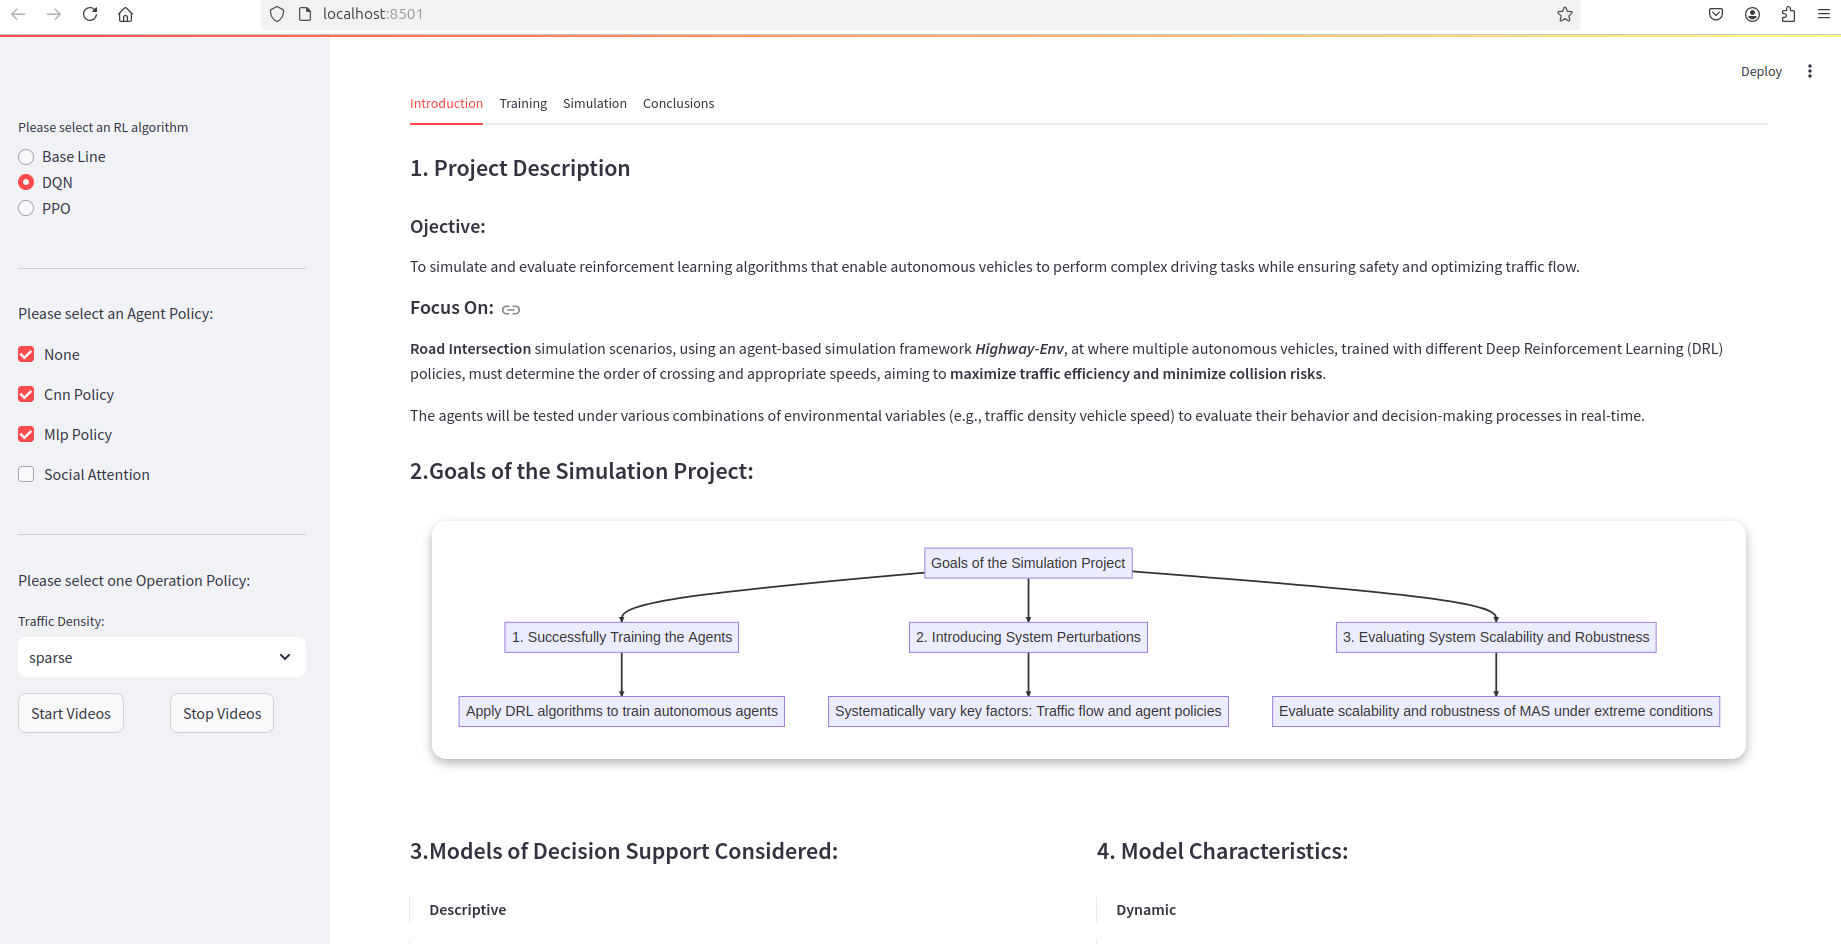
\includegraphics[height=0.35\textheight]{images/app_intro.png} 
    \caption{Streamlit Application - Layout}
\end{figure}


\subsection{Streamlit Application for RL Highway-Env}

The Streamlit application implements the functionality for simulating and analyzing the performance of different agent policies in an intersection environment.
The main goal is to evaluate how the agent's policies perform under various traffic flow configurations, namely sparse and dense traffic. 
The key features and flow of the code are outlined as follows:

\subsubsection{Sidebar Configuration}

The sidebar is a crucial part of the application, allowing users to customize and select the simulation parameters. The sidebar is divided into several sections:

\begin{itemize}
    \item \textbf{RL Algorithm Selection:} 
    Users can select the reinforcement learning (RL) algorithm to be used for the simulation. The available options are:
    \begin{itemize}
        \item \textit{Base Line}
        \item \textit{DQN}
        \item \textit{PPO}
    \end{itemize}

    \item \textbf{Agent Policy Selection:} 
    The user can also select the policy for the agent from a set of options:
    \begin{itemize}
        \item \textit{None} 
        \item \textit{CNN Policy}
        \item \textit{MLP Policy}
        \item \textit{Social Attention}
    \end{itemize}
    
    \item \textbf{Traffic Density Selection:} 
    A dropdown menu lets the user select the traffic density configuration, which can either be:
    \begin{itemize}
        \item \textit{Sparse} (4 ego vehicles and a few other vehicles)
        \item \textit{Dense} (4 ego vehicles with many other vehicles)
    \end{itemize}

    \item \textbf{Video Control:} 
    The sidebar also includes two buttons to control the video playback of the simulation:
    \begin{itemize}
        \item \textit{Start Videos} - Starts the simulation videos
        \item \textit{Stop Videos} - Stops the simulation videos
    \end{itemize}
\end{itemize}

These options allow the user to specify the RL algorithm, agent policy, and traffic density, enabling them to test the performance of different configurations in the environment.

The application is also divided into several tabs, each serving a different purpose for presenting the simulation results and performance metrics. 
These tabs are as follows:

\begin{itemize}
    \item \textbf{Introduction Tab:} 
    This tab provides an overview of the application and its objectives. It introduces the simulation environment, the agent policies being evaluated, and the traffic configurations used for the experiments.
    
    \item \textbf{Training Tab:} 
    Here, users can explore the details of the training process. This section includes some theorethical basis of the train process as well as visualizations,graphs and plots of training results, such as mean rewards and loss functions, to help assess the agent's learning progress.
    
    \begin{figure}[H]
        \centering
        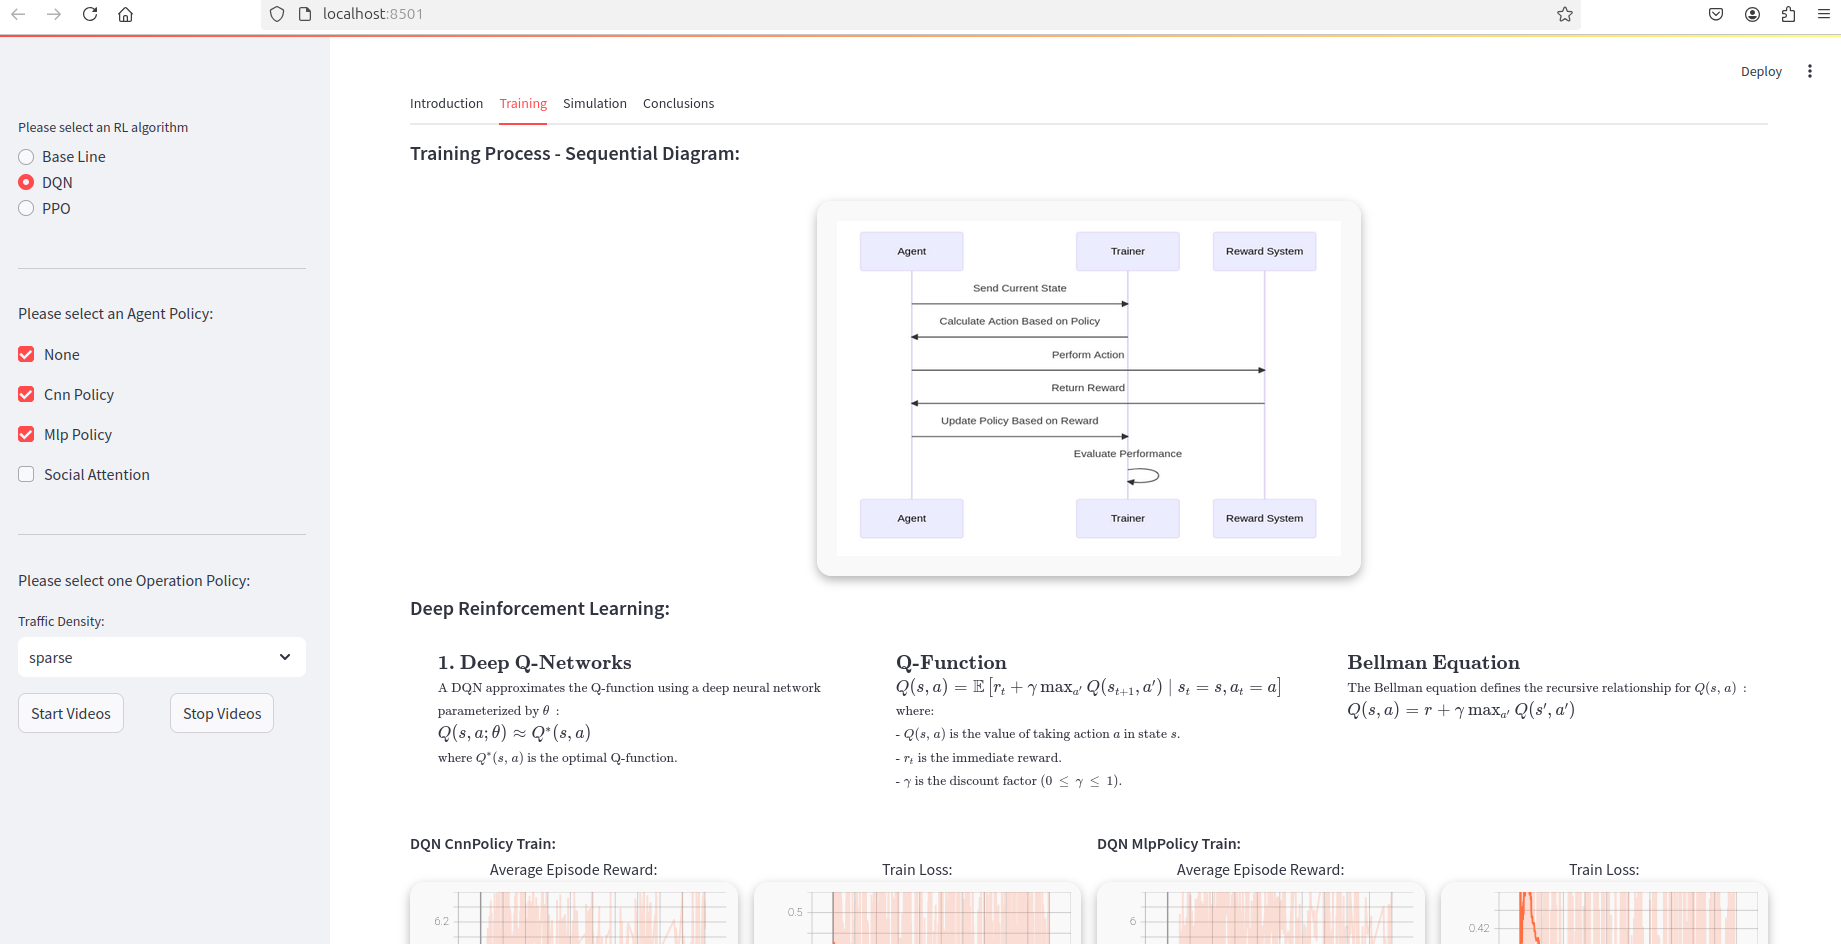
\includegraphics[height=0.35\textheight]{images/app_train.png} 
        \caption{Streamlit Application - Train Tab}
    \end{figure}
    

    \item \textbf{Simulation Tab:} 
    This tab shows the simulation results based on the selected agent policy, algorithm, and traffic configuration. The user can view simulation videos, performance plots, and metrics related to the agent's interaction with the environment.
    
  
    \begin{figure}[H]
        \centering
        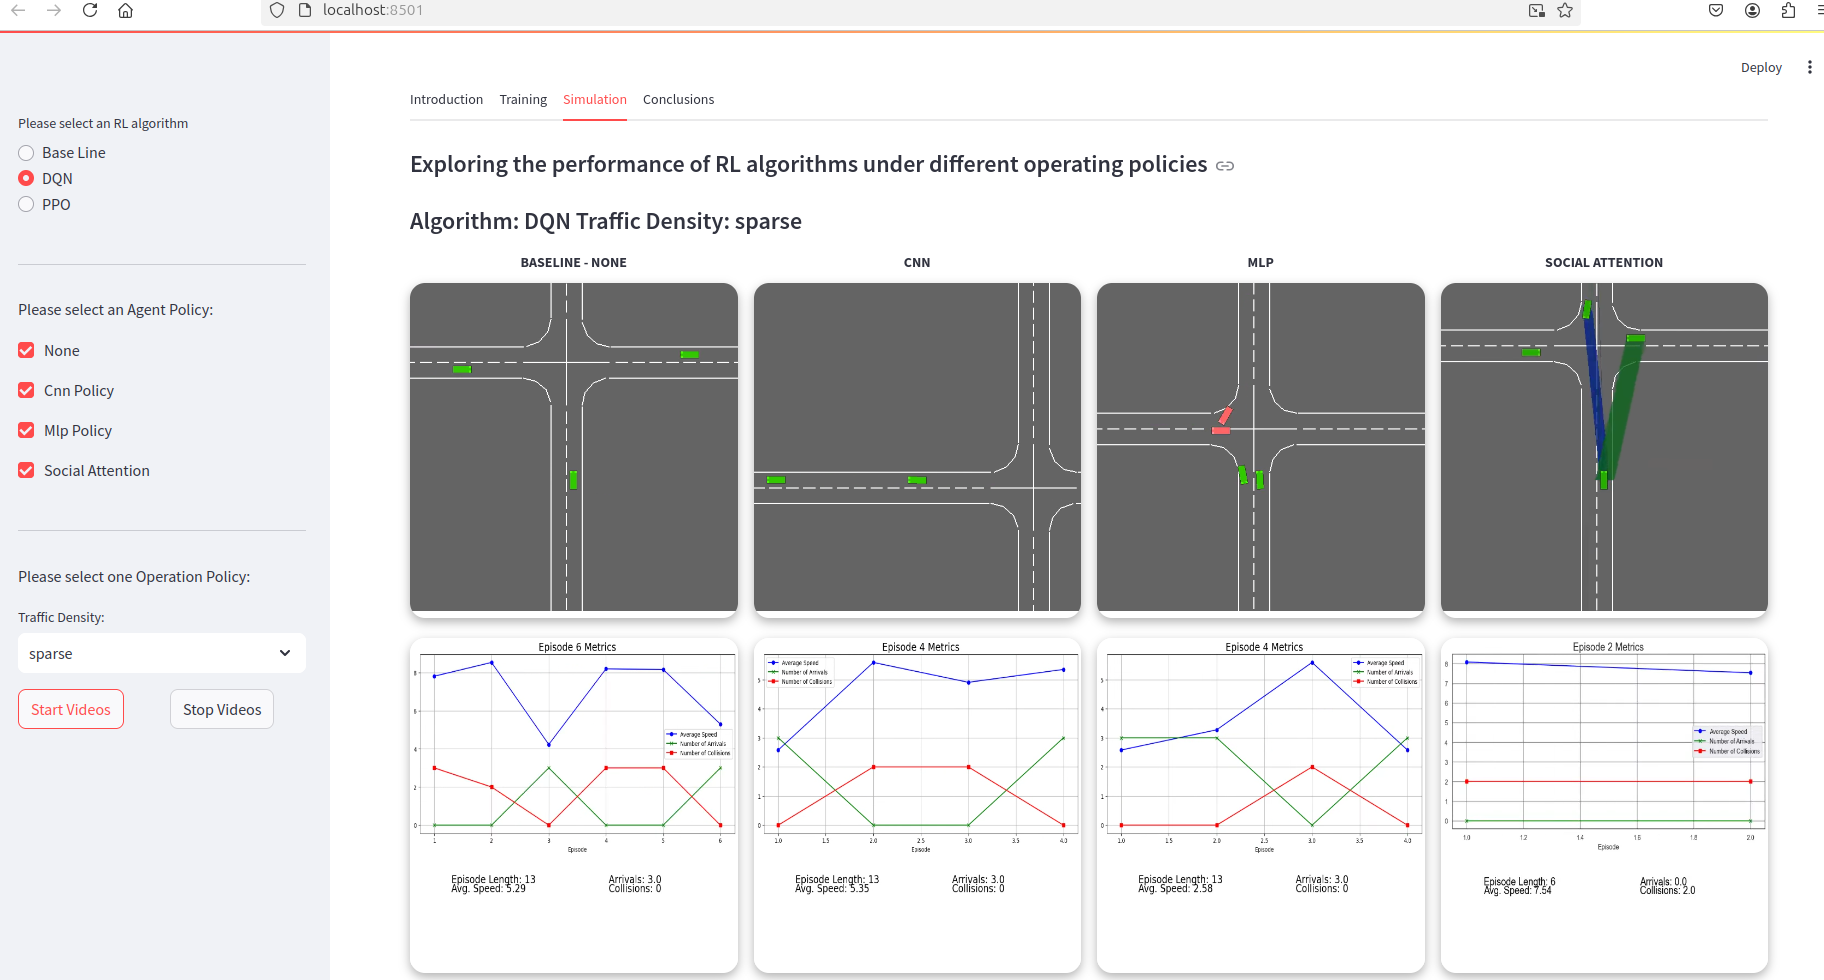
\includegraphics[height=0.35\textheight]{images/app_simulation.png} 
        \caption{Streamlit Application - Simulation Tab}
    \end{figure}
    

    \item \textbf{Conclusions Tab:} 
    This section summarizes the findings of the experiments, discusses the agent's performance under various configurations, and highlights any insights derived from the evaluation.
\end{itemize}

\begin{figure}[H]
    \centering
    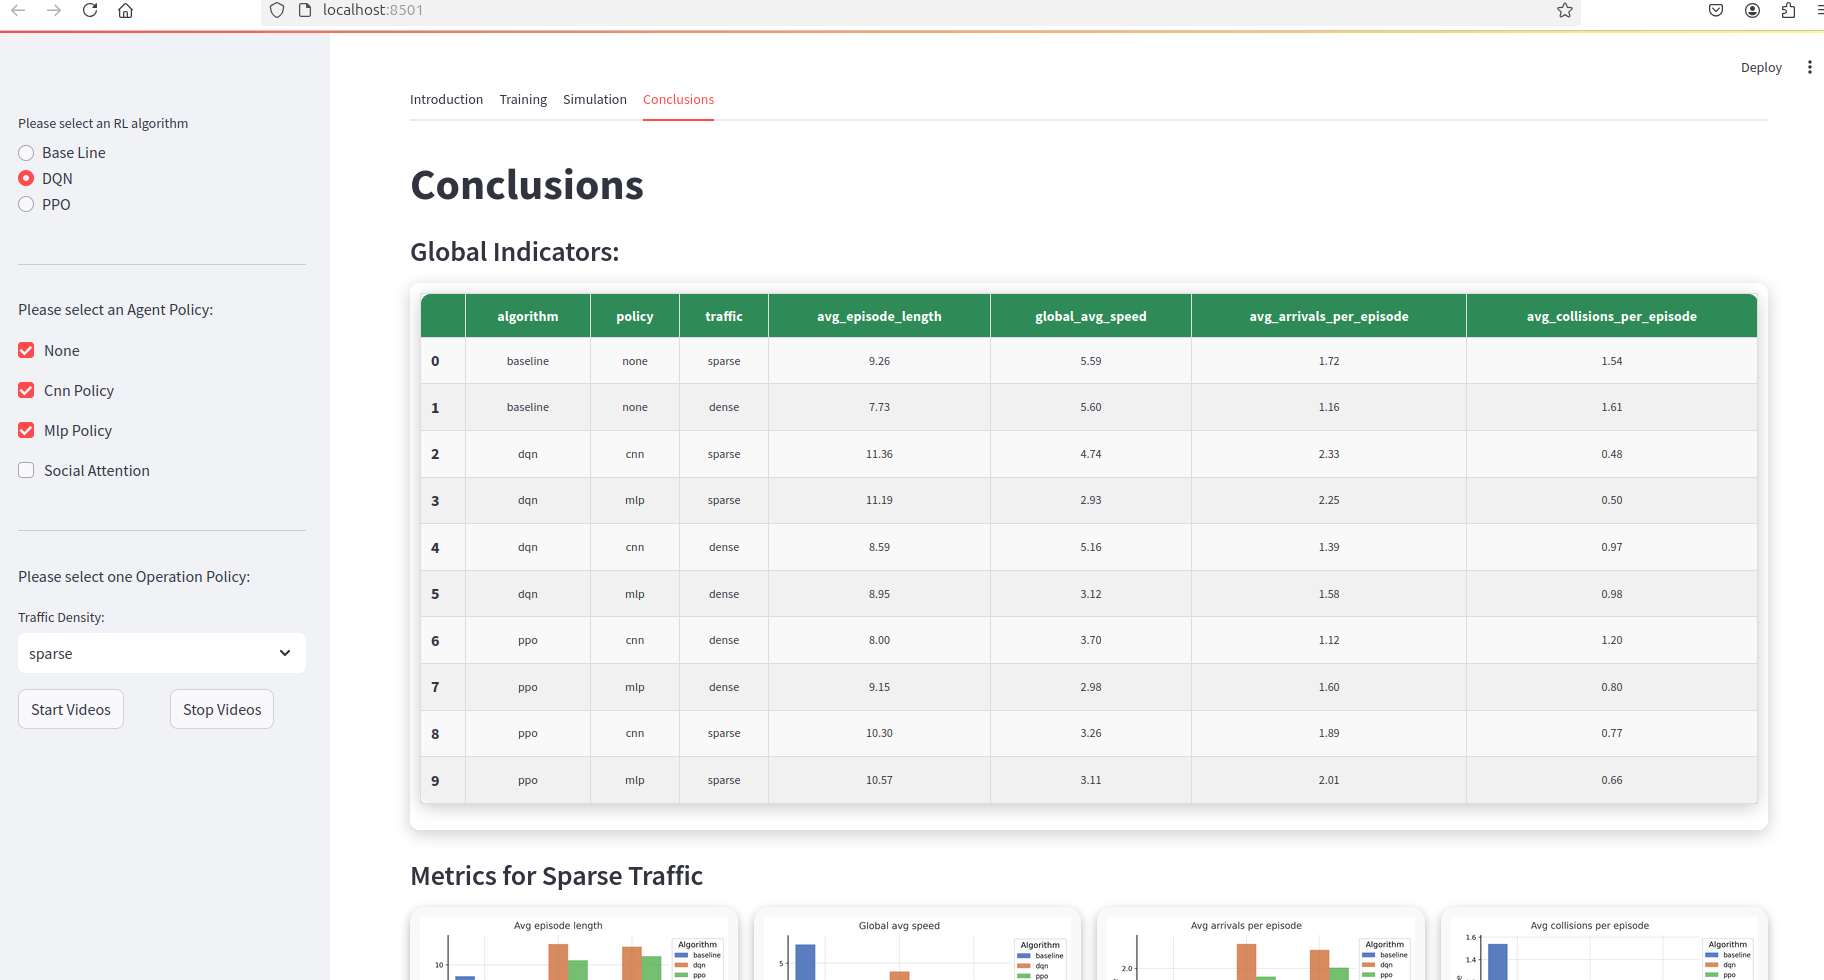
\includegraphics[height=0.35\textheight]{images/app_conclusions.png} 
    \caption{Streamlit Application - Conclusions Tab}
\end{figure}

\newpage

\section{Evaluate system scalability and robustness}

After training the learning models and integrating them into the application, we will utilize the approximated policy to inform decision-making. 

We conduct \textbf{100 simulations} for each algorithm or policy, collecting metrics from the environment based on this policy. 
These metrics allow us to evaluate the performance of the trained model and environment:
\begin{itemize}
    \item \textbf{Local metrics} give insight into the performance of the model within individual episodes, such as how efficiently it minimizes collisions or maximizes arrivals.
    \item \textbf{Global metrics} summarize the overall performance of the model across multiple episodes, useful for comparing different algorithms, policies, or configurations.
\end{itemize}

\subsection{Metrics Description}

\subsubsection*{Local Metrics (per episode)}

\begin{enumerate}
    \item \textbf{Average Speed}:
    \begin{itemize}
        \item \textbf{Description}: The average speed of all agents in the environment during the current episode.
        \item \textbf{Formula}:
        \[
        \text{avg\_speed} =
        \begin{cases}
        \frac{\text{speed\_sum}}{\text{step\_count}}, & \text{if } \text{step\_count} > 0 \\
        0, & \text{otherwise}
        \end{cases}
        \]
    \end{itemize}
    
    \item \textbf{Total Arrived Reward}:
    \begin{itemize}
        \item \textbf{Description}: The cumulative reward for all agents arriving at their destinations during the episode.
        \item \textbf{Formula}:
        \[
        \text{total\_arrived\_reward} = \text{infos}["\text{rewards}"]["\text{arrived\_reward}"]
        \]
        (Directly fetched from the environment's information dictionary).
    \end{itemize}
    
    \item \textbf{Number of Arrivals}:
    \begin{itemize}
        \item \textbf{Description}: The number of vehicles that successfully arrived at their destination in the current episode. 
       
        Each arrival contributes a reward of \(\frac{1}{\text{number\_of\_controlled\_agents}}\), so the number of arrivals is calculated by dividing 
        the total arrived reward by that fraction.

        \item \textbf{Formula}:
        \[
        \text{number\_of\_arrivals} = \frac{\text{total\_arrived\_reward}}{\frac{1}{\text{number\_of\_controlled\_agents}}}
        \]
    \end{itemize}
    
    \item \textbf{Number of Collisions}:
    \begin{itemize}
        \item \textbf{Description}: The number of collisions that occurred during the episode. This is inferred by summing the termination flags of agents (if provided by the environment).
        \item \textbf{Formula}:
        \[
        \text{number\_of\_collisions} = \sum \text{infos}["\text{agents\_terminated}"]
        \]
        (Assumes the termination flag indicates a collision).
    \end{itemize}
\end{enumerate}

\subsubsection*{Global Metrics (across all episodes)}

\begin{enumerate}
    \item \textbf{Global Average Speed}:
    \begin{itemize}
        \item \textbf{Description}: The overall average speed of all agents across all episodes.
        \item \textbf{Formula}:
        \[
        \text{global\_avg\_speed} =
        \begin{cases}
        \frac{\text{total\_speed\_sum}}{\text{total\_step\_count}}, & \text{if } \text{total\_step\_count} > 0 \\
        0, & \text{otherwise}
        \end{cases}
        \]
    \end{itemize}
    
    \item \textbf{Average Arrivals per Episode}:
    \begin{itemize}
        \item \textbf{Description}: The mean number of vehicles that successfully arrived at their destinations per episode.
        \item \textbf{Formula}:
        \[
        \text{avg\_arrivals\_per\_episode} = \frac{\text{total\_arrivals}}{\text{n\_episodes}}
        \]
    \end{itemize}
    
    \item \textbf{Average Collisions per Episode}:
    \begin{itemize}
        \item \textbf{Description}: The mean number of collisions that occurred per episode.
        \item \textbf{Formula}:
        \[
        \text{avg\_collisions\_per\_episode} = \frac{\text{total\_collisions}}{\text{n\_episodes}}
        \]
    \end{itemize}
    
    \item \textbf{Average Episode Length}:
    \begin{itemize}
        \item \textbf{Description}: The mean number of steps (time steps) per episode.
        \item \textbf{Formula}:
        \[
        \text{avg\_episode\_length} = \frac{\text{total\_step\_count}}{\text{n\_episodes}}
        \]
    \end{itemize}
\end{enumerate}

\subsection{Metrics Collection}

The metrics are collected during the environment simulation loop, specifically in the section where the step() function of the environment is called. 

\begin{lstlisting}[style=python]
obs, reward, terminated, truncated, infos = env.step(action)
\end{lstlisting}


The \texttt{step()} function takes the action predicted by the model and advances the environment by one time step. The outputs are:
\begin{itemize}
    \item \texttt{obs}: The new observation (state) after taking the action.
    \item \texttt{reward}: The immediate reward from the environment for the action.
    \item \texttt{terminated}: A boolean indicating if the episode has ended due to termination criteria.
    \item \texttt{truncated}: A boolean indicating if the episode has ended due to a time limit.
    \item \texttt{infos}: A dictionary containing additional information from the environment.
\end{itemize}

After each step, the \texttt{infos} dictionary is used to update various metrics:

\begin{verbatim}
speed_sum += infos['speed']
\end{verbatim}
The speed of the agents at this time step is fetched from the \texttt{infos} dictionary and added to \texttt{speed\_sum}. This accumulates the total speed over the episode.

\begin{verbatim}
step_count += 1
\end{verbatim}
The \texttt{step\_count} variable is incremented with each step to keep track of the number of steps in the episode.

At the end of the episode (when \texttt{terminated} or \texttt{truncated} is \texttt{True}), additional metrics are calculated:

\begin{verbatim}
avg_speed = speed_sum / step_count if step_count > 0 else 0
\end{verbatim}
The total speed accumulated during the episode is divided by the total steps to calculate the average speed.

\begin{verbatim}
total_arrived_reward = infos["rewards"]["arrived_reward"]
number_of_arrivals = total_arrived_reward / (1/number of controlled vehicles)
\end{verbatim}
The total arrived reward is fetched directly from the \texttt{infos} dictionary, and the number of arrivals is derived by dividing this reward by \(0.25\).

\begin{verbatim}
if not truncated:
    final_agents_terminated = infos["agents_terminated"]
    number_of_collisions = sum(final_agents_terminated)
\end{verbatim}
If the episode ended due to termination, the \texttt{agents\_terminated} information from the \texttt{infos} dictionary is used to infer the number of collisions.



The \textbf{global metrics} are computed by aggregating and averaging data collected across all episodes. 

These metrics provide insights into the overall performance of the model.

\begin{itemize}
\item\textbf{Global Average Speed}:The overall average speed of all agents across all episodes.  
\begin{verbatim}
global_avg_speed = total_speed_sum / total_step_count if total_step_count > 0 else 0
\end{verbatim}

\item\textbf{Average Arrivals per Episode} The mean number of vehicles that successfully arrived at their destinations per episode. 
\begin{verbatim}
avg_arrivals_per_episode = total_arrivals / n_episodes
\end{verbatim}


\item\textbf{Average Collisions per Episode} The mean number of collisions that occurred per episode. 
\begin{verbatim}
avg_collisions_per_episode = total_collisions / n_episodes
\end{verbatim}


\item\textbf{Average Episode Length} The mean number of steps (time steps) per episode.
\begin{verbatim}
avg_episode_length = total_step_count / n_episodes
\end{verbatim}
\end{itemize}

These metrics are stored and optionally exported to a CSV file for further analysis. 

They allow for evaluating and comparing the performance of different algorithms, policies, or traffic configurations:
\begin{itemize}
    \item \textbf{Global Average Speed:} Indicates how effectively the model maintains higher speeds across episodes.
    \item \textbf{Average Arrivals per Episode:} Measures how successfully the agents reach their destinations.
    \item \textbf{Average Collisions per Episode:} Tracks the frequency of collisions, highlighting safety concerns.
    \item \textbf{Average Episode Length:} Provides insight into the time efficiency of episodes. Longer episodes means better model performance.
\end{itemize}

During the simulation, the application generates and displays separate plots for the local metrics, enabling a visual comparison of the different algorithms and policies selected by the user. 


\begin{figure}[H]
    \centering
    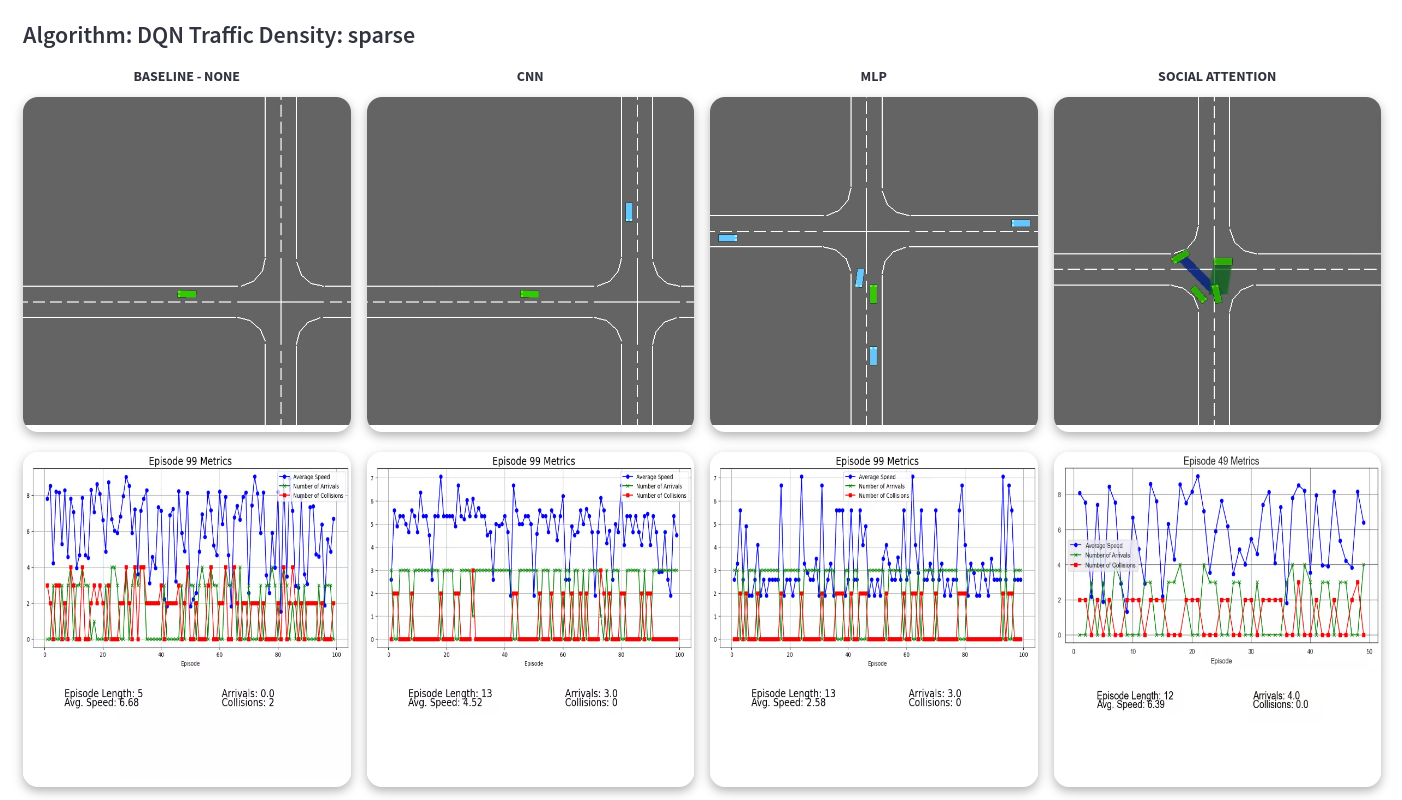
\includegraphics[height=0.4\textheight]{images/app_plots.png} 
    \caption{Simulation - Local Metrics Plot}
\end{figure}

At the conclusion of all episodes, the global metrics for each scenario can also be presented.

\begin{figure}[H]
    \centering
    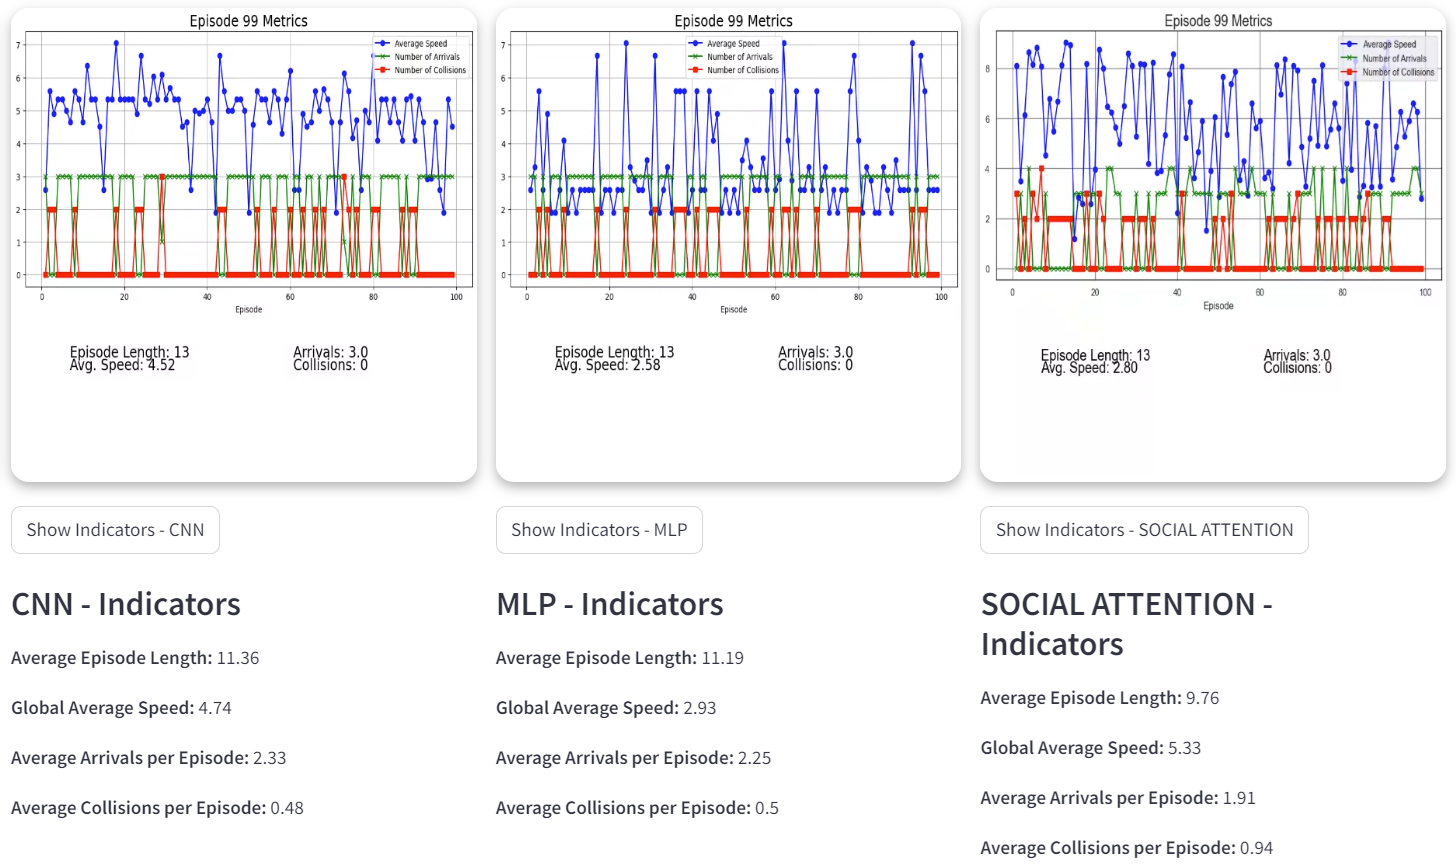
\includegraphics[height=0.4\textheight]{images/app_global_metrics.png} 
    \caption{Simulation - Global Metrics}
\end{figure}


\subsection{Performance Indicators}

Based on the global metrics obtained from the simulation results, we will classify the performance of the different algorithm/policy combinations according to three categories: Efficiency, Safety, and Adaptability. 

In this analysis we will use the following indicators:

\subsubsection{Traffic Flow Efficiency}

\textbf{Average Speed per Arrived Vehicle} 

\[
\text{Efficiency} = \frac{\text{Average Speed}}{\text{Average Arrivals per Episode}}
\]

Dividing the overall speed by the number of arrived vehicles gives a sense of how fast vehicles are reaching their destinations. Higher values indicate not only a good throughput but also timely arrivals.

\subsubsection{Safety Indicators}

\textbf{Collision Rate per 100 Steps} 

\[
\text{Collision Rate} = \frac{\text{Average Collisions per Episode}}{\text{Average Episode Length}} \times 100
\]

Normalizing the collision count by the episode length accounts for varying durations of simulations, making it easier to compare safety across different scenarios or environments. Reporting collisions per 100 steps provides a standardized and interpretable safety metric.


\textbf{Efficiency-to-Safety Tradeoff Index}
\[
\text{Tradeoff Index} = \frac{\text{Average Speed per Arrived Vehicle}}{\text{Collision Rate per 100 Steps}}
\]

This indicator balances the system's efficiency (how fast vehicles are moving and arriving) against its safety (collision rate).




\subsubsection{Adaptability to Varying Traffic Conditions}

\textbf{Relative Variance in Throughput}
\[
\text{Adaptability} = \frac{\text{Variance(Throughput)}}{\text{Mean(Throughput)}}
\]

The relative variance of throughput under different traffic densities captures the system's stability. Lower relative variance indicates consistent performance, even under fluctuating conditions.



\textbf{Traffic Load Adaptability} 
Compare throughput or wait times between low and high-density traffic scenarios, e.g.:
\[
\text{Load Adaptability} = \frac{\text{Throughput (High Density)}}{\text{Throughput (Low Density)}}
\]

This measures how well the system scales and maintains performance as traffic density increases.


\textbf{Safety Margins Under Stress}
\[
\text{Stress Safety Index} = \frac{\text{Collision Rate (High Density)}}{\text{Collision Rate (Low Density)}}
\]

Quantifying how safety degrades under heavier traffic loads provides insights into the robustness of safety mechanisms.


We will categorize each metric (Efficiency, Safety, and Adaptability) into High, Medium, and Low categories for each algorithm-policy pair.

\begin{itemize}
    \item \textbf{Efficiency (Average Speed per Arrived Vehicle):}
    \begin{itemize}
        \item High: Top 33\% of values
        \item Medium: Middle 33\% of values
        \item Low: Bottom 33\% of values
    \end{itemize}

    \item \textbf{Safety (Collision Rate per 100 Steps):}
    \begin{itemize}
        \item High: Lowest 33\% of values (lower collision rate is better)
        \item Medium: Middle 33\% of values
        \item Low: Highest 33\% of values (higher collision rate is worse)
    \end{itemize}

    \item \textbf{Adaptability (Adaptability, Load Adaptability, Stress Safety Index):}
    \begin{itemize}
        \item High: Lowest 33\% of adaptability values
        \item Medium: Middle 33\% of values
        \item Low: Highest 33\% of adaptability values (greater variance means lower adaptability)
    \end{itemize}
\end{itemize}

These indicators are classified using quantiles (33\%, 67\%) to categorize them into High, Medium, and Low categories.

